\documentclass[uplatex,dvipdfmx]{beamer}
\usepackage{listings,jvlisting}
\usepackage{color}
\usepackage{xr}

\lstset{
  backgroundcolor=\color[rgb]{0.9,0.9,0.9},
  frame=single,
  basicstyle=\ttfamily
}
\makeatletter
\newcommand*{\addFileDependency}[1]{% argument=file name and extension
  \typeout{(#1)}
  \@addtofilelist{#1}
  \IfFileExists{#1}{}{\typeout{No file #1.}}
}
\makeatother

\newcommand*{\myexternaldocument}[1]{%
    \externaldocument{#1}%
    \addFileDependency{#1.tex}%
    \addFileDependency{#1.aux}%
}
\myexternaldocument{../categoryTheoryIntro/CategoryTheoryIntro}

\newcommand{\pr}[1]{\colorbox[rgb]{0.9,0.9,0.9}{\lstinline{#1}}}
\newcommand{\functype}[2]{\pr{#1 -> #2}}
\newcommand{\refcti}[1]{\cite{cti}\ref{#1}}
\newcommand{\fpmor}[3]{\pr{#1 :: #2 -> #3}}
\usefonttheme[onlymath]{serif}

\usepackage{tikz}
\usepackage{bbm}
\usepackage{amsmath,amssymb}
\usepackage{url}
\usetikzlibrary{matrix,arrows}

\newcommand{\cat}[1]{\mathbbm{#1}}
\newcommand{\arrow}{\rightarrow}
\newcommand{\functor}[3]{#1:\cat{#2}\arrow \cat{#3}}
\newcommand{\profunctor}[3]{#1:\cat{#2}\nrightarrow \cat{#3}}

\newcommand{\nat}[3]{#1:#2\Rightarrow #3}
\newcommand{\natf}[5]{#1:#2\Rightarrow #3:\cat{#4}\arrow \cat{#5}}
\newcommand{\tuple}[1]{\langle #1\rangle}
\newcommand{\objr}[1]{\mathrm{Obj}(#1)}
\newcommand{\obj}[1]{\mathrm{Obj}(\cat{#1})}
\newcommand{\morset}[1]{\mathrm{Mor}(\cat{#1})}

\newcommand{\mor}[3]{#1:#2\arrow #3}
\newcommand{\dom}{\mathrm{dom}}
\newcommand{\cod}{\mathrm{cod}}
\newcommand{\arset}[3]{\cat{#1}(#2,#3)}
\newcommand{\arsetr}[3]{#1(#2,#3)}
\newcommand{\pcobj}[1]{[#1]}
\newcommand{\funccat}[2]{\cat{#2}^\cat{#1}}

\newcommand{\coend}[2]{\displaystyle\int^{#2:\cat{#1}}\!\!\!\!\!\!\!}
\newcommand{\cend}[2]{\displaystyle\int_{#2:\cat{#1}}\!\!\!\!\!\!\!}
\newcommand{\natlat}[3]{\{#1\}_{#3\in #2}}
\newcommand{\inset}[2]{[#1,#2]}
\newcommand{\incat}[2]{[\cat{#1},\cat{#2}]}
\newcommand{\incatp}[2]{[#1,#2]}

\newenvironment{mydescription}
{\begin{description}
  \setlength{\parskip}{0.5cm}
}
{\end{description}}
\title{プロファンクターオプティクスの理論と実装}
\usetheme{Madrid}
\setbeamertemplate{navigation symbols}{}
\begin{document}
  \begin{frame}
    \titlepage
  \end{frame}
  \begin{frame}\frametitle{目的}

    データへのアクセサの一般化であるLensやキャストの一般化であるPrismは更にOpticsという概念へと一般化される。\\
    \vspace{\baselineskip}

    これらの一般化には圏論が用いられるが、興味深いことに圏論は自身を抽象化できる。そのためOpticも更に一般化できると考えた。    
  \end{frame}
  \begin{frame}\frametitle{全体の構成}
    \begin{itemize}
      \item 最初に導入として比較的身近なLensとPrismを紹介し、Opticを定義してOpticがそれらの一般化であることを示す。\\
      \vspace{\baselineskip}
      \item 次に丹原加群を定義して、Opticとの関係性を丹原Double圏同値として示す。\\
      \vspace{\baselineskip}
      \item そして最後にこれらの主要な結果として、Opticの別の形態を与えるプロファンクターの表現定理を述べる。
    \end{itemize}
  \end{frame}
  \begin{frame}\frametitle{データアクセサの一般化Lens}
    \begin{definition}[Lens\cite{categories_of_optics}]
      Lensは以下の二つの写像で構成される。
      \[\mor{\mathrm{get}}{S}{A},\ \mor{\mathrm{put}}{S\times A'}{S'}\]
    \end{definition}
    ここで$S:=B\times A,\ S':=B\times A'$とすると、
    \begin{alignat*}{7}
      \mathrm{get}:\ &S\ &\longrightarrow \ &A \ \ \ &\mathrm{put}:\ &S\times A'\ &\longrightarrow \ &S'\\
      &\tuple{b,a}&\longmapsto\ &a      &&\tuple{\tuple{b,a},a'}&\longmapsto\ &\tuple{b, a'}
    \end{alignat*}
    またこのような二つの写像の組の全体を$\mathrm{Lens}(A,A',S,S')$とする。すなわち\[\mathrm{Lens}(A,A',S,S') := \inset{S}{A}\times \inset{S\times A'}{S'}\]となる。($\inset{A}{B}$は集合$A$から$B$への写像の集合とする。)
  \end{frame}
  \begin{frame}\frametitle{キャストの一般化Prism}
    \begin{definition}[Prism\cite{categories_of_optics}]
      Prismは以下の二つの射で構成される。
      \[\mor{\mathrm{downcast}}{S}{S' + A},\ \mor{\mathrm{upcast}}{A'}{S'}\]
    \end{definition}
    ここで$S:=B+ A,\ S':=B+ A'$とすると、
    \begin{alignat*}{20}
      \mathrm{downcast}:\ &S\ \ &\longrightarrow \ \ &S'+&A & \ \ \ \ \mathrm{upcast}: &A'&\longrightarrow &\ S'\\
      &a \ \ &\longmapsto \ \ &&a &&a'&\longmapsto &a'\\
      &b \ \ &\longmapsto \ \ &b& &
    \end{alignat*}
    Lensと同様に\[\mathrm{Prism}(A,A',S,S') := \inset{S}{S'+A}\times\inset{A'}{S}\]とする。
  \end{frame}
  \begin{frame}\frametitle{LensとPrismの双対性}
    \begin{theorem}
     LensとPrismは双対である。
    \end{theorem}
    \vspace{\baselineskip}
    二つの概念が双対であるとは、それを構成する射の向きがすべて逆であることである。例えば積と余積はどちらも以下の図式によって定義される。
    {\tiny
    \begin{center}
      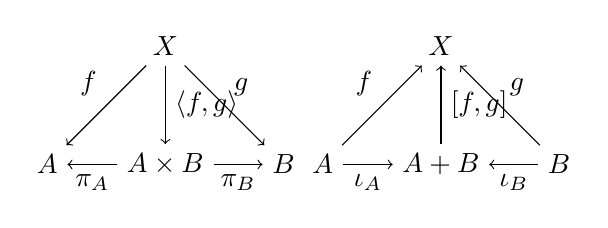
\begin{tikzpicture}[auto]
        \node (X) at (0, 1.5) {$X$};
        \node (AB) at (0, 0) {$A\times B$};
        \node (A) at (-1.5, 0) {$A$};
        \node (B) at (1.5, 0) {$B$};

        \draw[->] (X) to node[swap]{$f$}(A);
        \draw[->] (X) to node{$g$}(B);
        \draw[->] (AB) to node{$\pi_A$}(A);
        \draw[->] (AB) to node[swap]{$\pi_B$}(B);
        \draw[->] (X) to node{$\tuple{f,g}$}(AB);

        \node (X) at (3.5, 1.5) {$X$};
        \node (AB) at (3.5, 0) {$A+B$};
        \node (A) at (2, 0) {$A$};
        \node (B) at (5, 0) {$B$};

        \draw[<-] (X) to node[swap]{$f$}(A);
        \draw[<-] (X) to node{$g$}(B);
        \draw[<-] (AB) to node{$\iota_A$}(A);
        \draw[<-] (AB) to node[swap]{$\iota_B$}(B);
        \draw[<-] (X) to node{$[f,g]$}(AB);
      \end{tikzpicture}
    \end{center}}
    これによってLens\ $\inset{S}{A}\times \inset{S\times A'}{S'}$とPrism\ $\inset{S}{S'+A}\times\inset{A'}{S}$が双対の関係にあると分かる。
  \end{frame}
  \begin{frame}\frametitle{Opticの定義}
    \begin{definition}[Optic\cite{categories_of_optics}]
      四つの集合$A,A',S,S'$に対するOpticの集合を\[\mathrm{Optic}(A,A',S,S') := \int^M \inset{S}{M\otimes A}\times \inset{M\otimes A'}{S'}\]と定義する。
    \end{definition}
    \begin{mydescription}
      \item[モノイダル積$\otimes$] 直積$\times$、直和$+$の一般化した演算である。\\
      また集合のみならず写像のモノイダル積も取ることができる。つまり二つの写像$\mor{f}{A}{B},\ \mor{g}{C}{D}$を合成した写像
      \[\mor{f\otimes g}{A\otimes C}{B\otimes D}\]が得られる。
      \item[コエンド$\int^M$] 対象$M$を添字とする直和集合を取る操作。
    \end{mydescription}
  \end{frame}
  \begin{frame}\frametitle{ストリングダイアグラム}
    モノイダル積の並列性$\mor{f\otimes g}{A\otimes C}{B\otimes D}$を以下のように表す。
    \begin{center}
      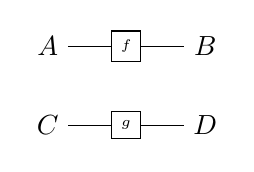
\begin{tikzpicture}
        \node (A) at (0, 0) {$A$};
        \node (B) at (2, 0) {$B$};
        \node (C) at (0, -1) {$C$};
        \node (D) at (2, -1) {$D$};
        \draw[-] (A) to node[draw, fill=white]{\tiny{$f$}}(B);
        \draw[-] (C) to node[draw, fill=white]{\tiny{$g$}}(D);
      \end{tikzpicture}
    \end{center}
    すると$\int^M \inset{S}{M\otimes A}\times \inset{M\otimes A'}{S'}$のある要素$\tuple{l,r}$は
    \begin{center}
      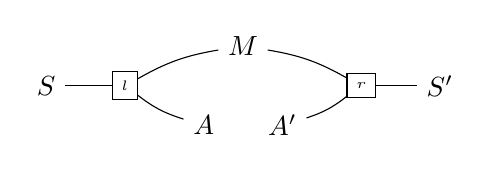
\begin{tikzpicture}
        \node (S) at (0, 0) {$S$};
        \node (M) at (2.5, 0.5) {$M$};
        \node (A) at (2, -0.5) {$A$};

        \node[draw] (l) at (1, 0) {{\tiny$l$}};
        \draw[-] (S) to (l);
        \draw[-] (l) to [bend left=10] (M);
        \draw[-] (l) to [bend right=10](A);

        \node (S') at (5, 0) {$S'$};
        \node (A') at (3, -0.5) {$A'$};
        \node[draw] (r) at (4, 0) {{\tiny$r$}};
        \draw[-] (r) to (S');
        \draw[-] (r) to [bend right=10] (M);
        \draw[-] (r) to [bend left=10](A');
      \end{tikzpicture}
    \end{center}
    と書くことができる。また$l,r$は本来独立な写像であるが、コエンドの性質より$M$につながる線をつなげて書くことができる。
  \end{frame}
  \begin{frame}
    \frametitle{LensはOpticである}
    モノイダル積$\otimes$が直積$\times$である時、
    \begin{center}
      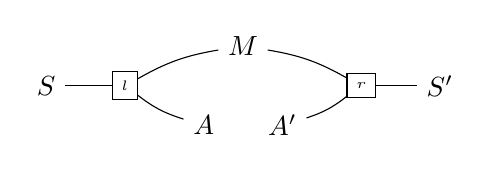
\begin{tikzpicture}
        \node (S) at (0, 0) {$S$};
        \node (M) at (2.5, 0.5) {$M$};
        \node (A) at (2, -0.5) {$A$};

        \node[draw] (l) at (1, 0) {{\tiny$l$}};
        \draw[-] (S) to (l);
        \draw[-] (l) to [bend left=10] (M);
        \draw[-] (l) to [bend right=10](A);

        \node (S') at (5, 0) {$S'$};
        \node (A') at (3, -0.5) {$A'$};
        \node[draw] (r) at (4, 0) {{\tiny$r$}};
        \draw[-] (r) to (S');
        \draw[-] (r) to [bend right=10] (M);
        \draw[-] (r) to [bend left=10](A');
      \end{tikzpicture}
    \end{center}
    $\inset{A}{B\times C}\cong\inset{A}{B}\times \inset{A}{C}$より、
    \begin{center}
      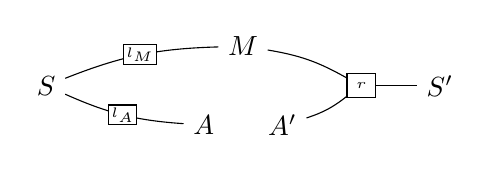
\begin{tikzpicture}
        \node (S) at (0, 0) {$S$};
        \node (M) at (2.5, 0.5) {$M$};
        \node (A) at (2, -0.5) {$A$};

        \draw[-] (S) to [bend left=10] node [draw,inner sep=1pt, fill=white]{\tiny$l_M$} (M);
        \draw[-] (S) to [bend right=10]node [draw,inner sep=1pt, fill=white]{\tiny$l_A$}(A);

        \node (S') at (5, 0) {$S'$};
        \node (A') at (3, -0.5) {$A'$};
        \node[draw] (r) at (4, 0) {{\tiny$r$}};
        \draw[-] (r) to (S');
        \draw[-] (r) to [bend right=10] (M);
        \draw[-] (r) to [bend left=10](A');
      \end{tikzpicture}
    \end{center}
    $FA\cong\int^M [A,M]\times FM$から
    \begin{center}
      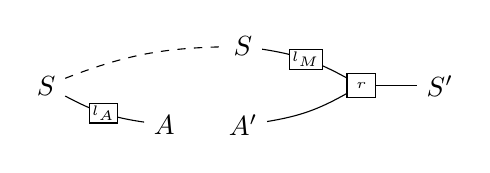
\begin{tikzpicture}
        \node (S) at (0, 0) {$S$};
        \node (A) at (1.5, -0.5) {$A$};
        \node (S2) at (2.5, 0.5) {$S$};
        \draw[-,dashed] (S) to [bend left=10] (S2);


        \draw[-] (S) to [bend right=10]node [draw,inner sep=1pt, fill=white]{\tiny$l_A$}(A);

        \node (S') at (5, 0) {$S'$};
        \node (A') at (2.5, -0.5) {$A'$};
        \node[draw] (r) at (4, 0) {{\tiny$r$}};
        \draw[-] (r) to (S');
        \draw[-] (r) to [bend right=10]node [draw,inner sep=1pt, fill=white]{\tiny$l_M$} (S2);
        \draw[-] (r) to [bend left=10](A');

      \end{tikzpicture}
    \end{center}
    よって$\mathrm{Optics}_\times(A,A',S,S') \cong \mathrm{Lens}(A,A',S,S')$
  \end{frame}
  \begin{frame}
    \frametitle{PrismはOpticである}
    モノイダル積$\otimes$が直和$+$である時、
    \begin{center}
      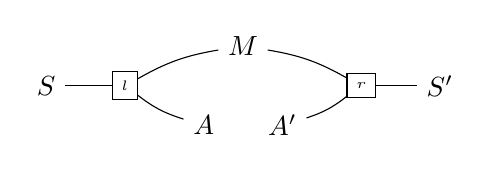
\begin{tikzpicture}
        \node (S) at (0, 0) {$S$};
        \node (M) at (2.5, 0.5) {$M$};
        \node (A) at (2, -0.5) {$A$};

        \node[draw] (l) at (1, 0) {{\tiny$l$}};
        \draw[-] (S) to (l);
        \draw[-] (l) to [bend left=10] (M);
        \draw[-] (l) to [bend right=10](A);

        \node (S') at (5, 0) {$S'$};
        \node (A') at (3, -0.5) {$A'$};
        \node[draw] (r) at (4, 0) {{\tiny$r$}};
        \draw[-] (r) to (S');
        \draw[-] (r) to [bend right=10] (M);
        \draw[-] (r) to [bend left=10](A');
      \end{tikzpicture}
    \end{center}
    $\inset{A+B}{C}\cong\inset{A}{C}+\inset{B}{C}$より、
    \begin{center}
      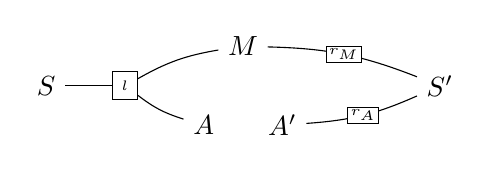
\begin{tikzpicture}
        \node (S) at (0, 0) {$S$};
        \node (M) at (2.5, 0.5) {$M$};
        \node (A) at (2, -0.5) {$A$};
        \node[draw] (l) at (1, 0) {{\tiny$l$}};
        \draw[-] (S) to (l);
        \draw[-] (l) to [bend left=10] (M);
        \draw[-] (l) to [bend right=10](A);

        \node (S') at (5, 0) {$S'$};
        \node (A') at (3, -0.5) {$A'$};
        \draw[-] (S') to [bend right=10] node [draw,inner sep=1pt, fill=white]{\tiny$r_M$} (M);
        \draw[-] (S') to [bend left=10]node [draw,inner sep=1pt, fill=white]{\tiny$r_A$}(A');
      \end{tikzpicture}
    \end{center}
    $FA\cong\int^M [M,A]\times FM$から
    \begin{center}
      \begin{tikzpicture}
        \node (S) at (0, 0) {$S$};
        \node (M) at (2.5, 0.5) {$S'$};
        \node (A) at (2.5, -0.5) {$A$};
        \node[draw] (l) at (1, 0) {{\tiny$l$}};
        \draw[-,dashed] (S') to [bend right=10] (M);

        \draw[-] (S) to (l);
        \draw[-] (l) to [bend left=10] (M);
        \draw[-] (l) to [bend right=10](A);

        \node (S') at (5, 0) {$S'$};
        \node (A') at (3.5, -0.5) {$A'$};
        \draw[-] (M) to [bend right=10] node [draw,inner sep=1pt, fill=white]{\tiny$r_M$} (l);
        \draw[-] (S') to [bend left=10]node [draw,inner sep=1pt, fill=white]{\tiny$r_A$}(A');
      \end{tikzpicture}
    \end{center}
    よって$\mathrm{Optics}_+(A,A',S,S') \cong \mathrm{Prism}(A,A',S,S')$
  \end{frame}

  \begin{frame}
    \frametitle{集合の圏}
    集合と写像の全体は圏と呼ばれる構造を持ち、これを$\cat{Set}$とする。\\
    \vspace{\baselineskip}
    \begin{definition}[集合の圏]
      {\small
      \begin{description}
        \item[対象] 任意の(小さい)集合を$\cat{Set}$の対象とする。
        \item[射] 対象$A,B$に対する射を任意の写像$\mor{f}{A}{B}$とする。
        \item[射の合成] 射の合成$f\circ g$はそのまま写像の合成とする。
      \end{description}
    }
    \end{definition}
  \vspace{\baselineskip}

  写像の集合は$\inset{A}{B}$で表せるが、これをOpticの集合$\mathrm{Optic}(A,A',S,S')$と置くと同様に圏が定義できる。
  \end{frame}
  \begin{frame}
    \frametitle{Opticの圏}
    \begin{definition}[Opticの圏\cite{categories_of_optics}]
      集合の圏上のOpticの圏を以下のように構成する。
      {\small
      \begin{description}
        \item[対象] 任意の(小さい)集合のニつ組を対象とする。
        \item[射] 対象$(A,A'),\ (S,S')$による射集合を$\mathrm{Optic}(A,A',S,S')$とする。
        \item[射の合成] 二つのOptic $\tuple{l',r'},\ \tuple{l,r}$の合成を$\tuple{(N\otimes l)\circ l',r'\circ(N\otimes r')}$とする。
      \end{description}
    }
    \end{definition}
    \begin{center}
      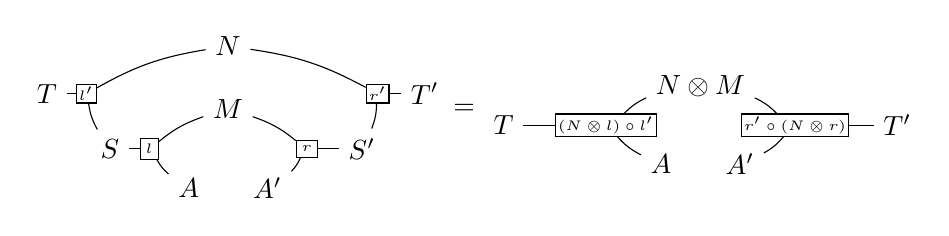
\begin{tikzpicture}
        \node (T) at (-0.8, 0.7) {$T$};

        \node (S) at (0, 0) {$S$};
        \node (M) at (1.5, 0.5) {$M$};
        \node (A) at (1, -0.5) {$A$};
        \node (N) at (1.5, 1.3) {$N$};

        \node[draw,inner sep=2pt] (l) at (0.5, 0) {{\tiny$l$}};

        \draw[-] (S) to (l);
        \draw[-] (l) to [bend left=10] (M);
        \draw[-] (l) to [bend right=10](A);
        \node[draw,inner sep=1pt] (l') at (-0.3, 0.7) {{\tiny$l'$}};
        \draw[-] (T) to (l');
        \draw[-] (l') to [bend right=10](S);
        \draw[-] (l') to [bend left=10] (N);

        \node (T') at (4, 0.7) {$T'$};
        \node (S') at (3.2, 0) {$S'$};
        \node (A') at (2, -0.5) {$A'$};
        \node[draw,inner sep=2pt] (r) at (2.5, 0) {{\tiny$r$}};
        \draw[-] (r) to (S');
        \draw[-] (r) to [bend right=10] (M);
        \draw[-] (r) to [bend left=10](A');

        \node[draw,inner sep=1pt] (r') at (3.4, 0.7) {{\tiny$r'$}};
        \draw[-] (T') to (r');
        \draw[-] (r') to[bend left=10] (S');
        \draw[-] (r') to [bend right=10] (N);

        \node (eq) at (4.5, 0.5) {$=$};

        \node (S) at (5, 0.3) {$T$};
        \node (M) at (7.5, 0.8) {$N\otimes M$};
        \node (A) at (7, -0.2) {$A$};

        \node[draw,inner sep=1pt] (l) at (6.3, 0.3) {{\tiny$(N\otimes l)\circ l'$}};
        \draw[-] (S) to (l);
        \draw[-] (l) to [bend left=10] (M);
        \draw[-] (l) to [bend right=10](A);

        \node (S') at (10, 0.3) {$T'$};
        \node (A') at (8, -0.2) {$A'$};
        \node[draw,inner sep=1pt] (r) at (8.7, 0.3) {{\tiny$r'\circ(N\otimes r)$}};
        \draw[-] (r) to (S');
        \draw[-] (r) to [bend right=10] (M);
        \draw[-] (r) to [bend left=10](A');
      \end{tikzpicture}
      \begin{tikzpicture}

      \end{tikzpicture}
    \end{center}
    またOpticの合成が定義できるので、Lens、Prismでも合成ができる。
  \end{frame}
  \begin{frame}
    \frametitle{丹原加群}

      \begin{definition}[丹原加群\cite{categories_of_optics}]
        丹原加群とは以下の図式を可換にするProfunctor $P$と射の族\[\mor{\zeta_{A,A',M}}{P(A,A')}{P(M\otimes A, M\otimes A')}\]の組$(P,\zeta)$である。
      {\tiny
      \begin{center}
        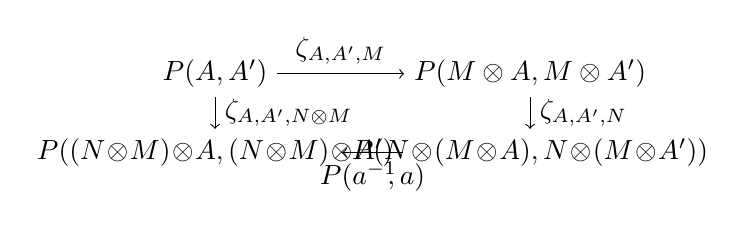
\begin{tikzpicture}[auto]
          \node (P) at (0, 0) {$P(A,A')$};
          \node (TP) at (4, 0) {$P(M\otimes A,M\otimes A')$};
          \node (TP2) at (0, -1) {$P((N\!\otimes\!M)\!\otimes\!A,(N\!\otimes\! M)\!\otimes\! A')$};
          \node (TTP) at (4, -1) {$P(N\!\otimes\! (M\!\otimes\! A),N\!\otimes\! (M\!\otimes\! A'))$};
          \draw[->] (P) to node{$\zeta_{A,A',M}$}(TP);
          \draw[->] (P) to node{$\zeta_{A,A',N\otimes M}$}(TP2);
          \draw[->] (TP) to node{$\zeta_{A,A',N}$}(TTP);
          \draw[->] (TP2) to node{$P(a^{-1}\!\!,a)$}(TTP);
        \end{tikzpicture}
        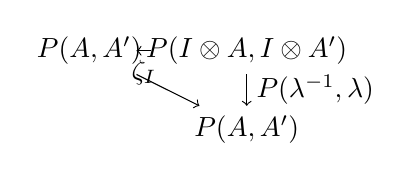
\begin{tikzpicture}[auto]
          \node (P) at (0, 0) {$P(A,A')$};
          \node (TP) at (2, 0) {$P(I\otimes A,I\otimes A')$};
          \node (P2) at (2, -1) {$P(A,A')$};
          \draw[->] (P) to node{$\zeta_I$}(TP);
          \draw[->] (TP) to node{$P(\lambda^{-1},\lambda)$}(P2);
          \draw[->] (P) to(P2);
        \end{tikzpicture}
      \end{center}}
      \end{definition}
      ただし、Profunctorは圏上の二項演算の一種である。
  \end{frame}
  \begin{frame}
    \frametitle{丹原加群の圏}
    \begin{definition}[丹原加群の圏\cite{categories_of_optics}]
      丹原加群の圏$\cat{Tamb}$を以下のように定義する。
      {\small
      \begin{description}
        \item[対象] 任意の丹原加群$(P,\zeta)$を対象とする。
        \item[射] 以下の図式を可換にする射の族$\mor{\alpha_{A,A'}}{P(A,A')}{Q(A,A')}$を射とする。\\
        {\tiny
          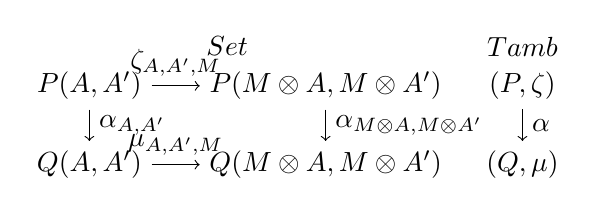
\begin{tikzpicture}[auto]
            \node (P) at (-1, 0) {$P(A,A')$};
            \node (Q) at (-1, -1) {$Q(A,A')$};
            \node (TP) at (2, 0) {$P(M\otimes A, M\otimes A')$};
            \node (TQ) at (2, -1) {$Q(M\otimes A, M\otimes A')$};
            \node (catpr) at (0.75, 0.5) {$\cat{Set}$};
  
            \draw[->] (P) to node{$\alpha_{A,A'}$}(Q);
            \draw[->] (P) to node{$\zeta_{A,A',M}$}(TP);
            \draw[->] (TP) to node{$\alpha_{M\otimes A,M\otimes A'}$}(TQ);
            \draw[->] (Q) to node{$\mu_{A,A',M}$}(TQ);
  
            \node (P) at (4.5, 0) {$(P,\zeta)$};
            \node (Q) at (4.5, -1) {$(Q,\mu)$};
            \draw[->] (P) to node{$\alpha$}(Q);
            \node (cattam) at (4.5, 0.5) {$\cat{Tamb}$};
  
          \end{tikzpicture}
          }
        \item[射の合成] 元の圏の射の合成からそのまま定義できる。
      \end{description}
      }
    \end{definition}
  \end{frame}
  \begin{frame}
    \frametitle{Opticの圏と丹原加群}
    丹原加群は$\cat{Optic}$から$\cat{Set}$への準同型写像と対応する。\\
    \vspace{\baselineskip}

    この対応は既存の文献において次の定理で知られているが、証明は行間が広いため定理の厳密化を行なった。
    \vspace{\baselineskip}

    \begin{theorem}[丹原Double圏同値\cite{profunctor_optics_update}\cite{doubles_for_monoidal}]
      \[\cat{Tamb}\simeq\incat{Optic}{Set}\]
      $\simeq$は圏の同型を緩めた等価性とし、$\incat{Optic}{Set}$は$\cat{Optic}$から$\cat{Set}$への準同型写像の成す圏である。
    \end{theorem}
    \vspace{\baselineskip}
  \end{frame}
  \begin{frame}\frametitle{Profunctor Optics}
    最後に最終目標であるProfunctorの表現定理を紹介する。
    \begin{theorem}[Profunctorの表現定理\cite{categories_of_optics}\cite{profunctor_optics_update}]
      \[\cat{Optic}(A,A',S,S') \cong \int_P \inset{P(A,A')}{P(S,S')}\]
      ただし$P$は任意の丹原加群とする。
    \end{theorem}
    \vspace{\baselineskip}

    本来$P$は丹原加群ではなく、$\cat{Optic}$から$\cat{Set}$の準同型写像であるが、前スライドの丹原Double圏同値によって丹原加群とみなせる。\\
    \vspace{\baselineskip}
    また左辺のような形で表したOpticをProfunctor Opticsと呼び、実用ではこちらを用いることが多い。
  \end{frame}
  \begin{frame}
    \frametitle{まとめ}
    \begin{itemize}
      \item LensとPrismを定義し、それらがOpticの一例であることを示した。
      \item 丹原加群を定義し、丹原Double圏同値によるOpticとの関係を示した。
      \item 丹原Double圏同値の応用として、Profunctorの表現定理を示した。
    \end{itemize}
    \vspace{\baselineskip}

    また具体的な成果として、丹原Double圏同値の定理の厳密化を行なった。

  \end{frame}
  \begin{frame}\frametitle{今後の課題}
    \begin{itemize}
      \item 2-圏論に関する体系的な知識を身につける。\\
      \vspace{\baselineskip}

      \item 2-圏論を用いて丹原Double圏同値の一貫した証明を示す。\\
      \vspace{\baselineskip}

      \item 丹原Double圏同値の一般化と思われる定理が2-圏論に存在するため、それとの関係を明らかにする。
    \end{itemize}
  \end{frame}
  \begin{frame}
    \frametitle{Opticの定義のさらなる一般化}
    このスライドではOpticを$\mathrm{Optic}(A,A',S,S'):=\int^M\inset{S}{M\otimes A}\times \inset{M\otimes A'}{S'}$と定義したが、論文のほうでは$\cat{Set}$で閉じることを要請せずに\[\int^M\arset{C}{S}{M\otimes A}\times \arset{C}{M\otimes A'}{S'}\]と定義している。さらに先行研究ではモノイダル積を圏への作用$\functor{\cdot}{M\times C}{C}$とした\[\int^M\arset{C}{S}{M\cdot A}\times \arset{C}{M\cdot  A'}{S'}\]なるOpticで議論される。またMixed Opticでは二つの射集合に現れる圏の作用のうち、それぞれ別の作用を用いている。
  \end{frame}
  \begin{frame}
    特にモノイダル積から作用への一般化では議論が複雑になってしまう。そのためそれらがもたらす良い性質を捨てることを覚悟し、次のOpticの定義を提唱する。ただし$\functor{F}{C}{C}$とする。
    \[\mathrm{FOptic(A,A',S,S')} := \int^F \arset{C}{S}{FA}\times \arset{C}{FA'}{S'}\]
    モノイダル積は$\mor{M \otimes -}{C}{C}$と表せ、$M$に関する射は自然変換で媒介できる。そのため明らかにOpticの拡張になっている。\\
    \vspace{\baselineskip}

    このFOpticを用いる利点として、異なるモノイダル積を採用したOptic同士を必ず合成できることがある。
  \end{frame}
  \begin{frame}
    \frametitle{FOpticとVan laarhoven encoding}
    FOpticを\[\mathrm{FOptic(A,A',S,S')} := \int^F \arset{C}{S}{FA}\times \arset{C}{FA'}{S'}\]と定義したが、Lens,Prismの異なる一般化としてVan laarhoven encodingがあり、\[\int_F \inset{\arset{C}{A}{FA}}{\arset{C}{S}{FS}}\]と定義される、構造が類似している。

    
  
  \end{frame}
  \begin{frame}
    \frametitle{Lens則}
    \begin{definition}[Lawful Lens\cite{categories_of_optics}]
      $\mathrm{Lens}(A,A,S,S)$の要素であり、以下の三つの図式を可換にする(get, put)をLawful Lensと呼ぶ。
    \begin{center}\scriptsize
      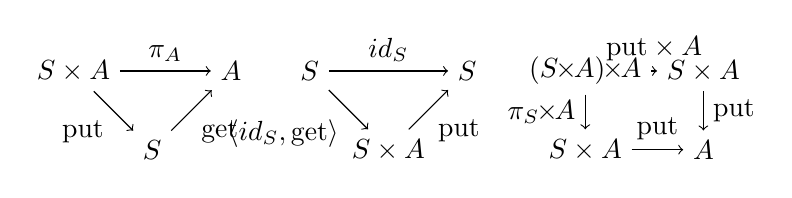
\begin{tikzpicture}[auto]
        \node (sa) at (0, 0) {$S\times A$};
        \node (s) at (1, -1) {$S$};
        \node (a) at (2, 0) {$A$};
        \draw[->] (sa) to node{$\pi_A$}(a);
        \draw[->] (sa) to node[swap]{$\mathrm{put}$}(s);
        \draw[->] (s) to node[swap]{$\mathrm{get}$}(a);

        \node (sa) at (3, 0) {$S$};
        \node (s) at (4, -1) {$S\times A$};
        \node (a) at (5, 0) {$S$};
        \draw[->] (sa) to node{$id_S$}(a);
        \draw[->] (sa) to node[swap]{$\tuple{id_S,\mathrm{get}}$}(s);
        \draw[->] (s) to node[swap]{$\mathrm{put}$}(a);

        \node (saa) at (6.5, 0) {$(S\!\!\times\!\! A)\!\!\times\!\! A$};
        \node (sa1) at (8, 0) {$S\times A$};
        \node (sa2) at (6.5, -1) {$S\times A$};
        \node (s) at (8, -1) {$A$};
        \draw[->] (saa) to node{$\mathrm{put}\times A$}(sa1);
        \draw[->] (saa) to node[swap]{$\pi_S\!\!\times \!\!A$}(sa2);
        \draw[->] (sa1) to node{$\mathrm{put}$}(s);
        \draw[->] (sa2) to node{$\mathrm{put}$}(s);
      \end{tikzpicture}
    \end{center}
    また図式による可換性をそれぞれputget、getput、putput則と呼ぶことにする。
    \end{definition}
    
    また同様に双対を取ることでLawful Prismも得られる。
  \end{frame}
  \begin{frame}
    \frametitle{Lawful Opti}
    LensがOpticへ一般化されるように、Lawful LensもまたLawful Opticへと一般化される。
    \begin{definition}[Lawful Opticc\cite{categories_of_optics}]
      以下の等式を満たすOptic $\tuple{l,r}$をLawful Opticと呼ぶ。
      \[r\circ l=id_S\]
      \[\tuple{l,\ l\circ r,\ r}=\tuple{l,\ id_{M\otimes A},\ r}\]

      ただし、二つ目の等式は集合{\scriptsize\[\mathrm{Optic}^2(A,A,S,S) = \int^{M,N} \inset{S}{M\otimes A}\times \inset{M\otimes A}{N\otimes A}\times \inset{N\otimes A}{S}\]}の上で成り立つとする。
    \end{definition}
  \end{frame}
  \begin{frame}
    \begin{theorem}[\cite{categories_of_optics}]
      あるLensがLawfulであることと、その一般化のOpticがLawfulであることは同値である。
    \end{theorem}
    $(\Longrightarrow)$についてはLens (get, put)をOpticに変換すると$\tuple{\tuple{id_S, \mathrm{get}}, \mathrm{put}}$となるから、\[\mathrm{put} \circ\tuple{id_S,\ \mathrm{get}} = id_S\]と、
    \[\tuple{\tuple{id_S,\ \mathrm{get}},\ \tuple{id_S,\ \mathrm{get}}\circ\mathrm{put},\ \mathrm{put}}=\tuple{\tuple{id_S,\ \mathrm{get}},\  id_{M\otimes A},\ \mathrm{put}}\]を示せばよい。
    どのように証明するか大まかに述べると、\\
    一つ目の等式は明らかにgetput則より成り立ち、二つ目の等式はputget則により中央のgetが消え、コエンドの性質より中央のputが左に移る。そしてputput則によりputが一つ消えて等式が成り立つ。
  \end{frame}
  \begin{frame}
    \frametitle{プロモナド}
    \begin{definition}
      Profunctor $\profunctor{M}{C}{C}\ (\functor{M}{C^{op}\times C}{Set})$によるモナド$(M,\mu,\eta)$を以下のように定義する。
      \begin{description}
        \item[乗算子] 自然変換$\nat{\mu}{M\diamond M}{M}$
        \item[単位子] 自然変換$\nat{\eta}{\arset{C}{-}{-}}{M}$
        \item[結合則単位則] 以下の二つの図式を可換にする。
        \begin{center}
          \tiny
          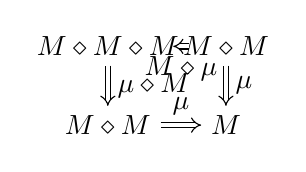
\begin{tikzpicture}[auto]
            \node (w) at (1.5, -1) {$M$};
            \node (ww) at (1.5, 0) {$M\diamond M$};
            \node (ww2) at (0, -1) {$M\diamond M$};
            \node (www) at (0, 0) {$M\diamond M\diamond M$};
            \draw[double,double equal sign distance,-implies] (ww) to node{$\mu$}(w);
            \draw[double,double equal sign distance,-implies] (ww2) to node{$\mu$}(w);
            \draw[double,double equal sign distance,-implies] (www) to node{$M\diamond \mu$}(ww);
            \draw[double,double equal sign distance,-implies] (www) to node{$\mu\diamond M$}(ww2);
          \end{tikzpicture}
          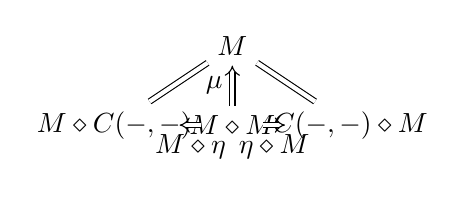
\begin{tikzpicture}[auto]
            \node (w) at (0, 0) {$M$};
            
            \node (ww) at (0, -1) {$M\diamond M$};
            \node (w2) at (-1.5, -1) {$M\diamond \arset{C}{-}{-}$};
            \node (w3) at (1.5, -1) {$\arset{C}{-}{-}\diamond M$};
            \draw[double,double equal sign distance,-implies] (ww) to node{$\mu$}(w);
            \draw[double,double equal sign distance,-implies] (w2) to node{$M\diamond\eta$}(ww);            
            \draw[double,double equal sign distance,-implies] (w3) to node[swap]{$\eta\diamond M$}(ww);

            \draw[double,double equal sign distance] (w) to (w2);
            \draw[double,double equal sign distance] (w) to (w3);

          \end{tikzpicture}
        \end{center}
      \end{description}
    \end{definition}
    ただし$(M\diamond M)(A,C) = \int^B M(B,C)\times M(A,B)$とする。\\
    また同様に自然変換の向きを入れ替えたプロコモナドも構成できる。
  \end{frame}
  \begin{frame}
    \frametitle{プロコモナドとLawful性}
    $\Phi(A,A,S,S)\ :=\ \mathrm{Optic}(A,A,S,S) = \int^M \inset{S}{M\otimes A}\times \inset{M\otimes A}{S}$とする。するとこれを以下のように関手とみなすことができる。\[\functor{\Phi}{C\times C^{op}\times C^{op}\times C}{Set}\]特に$\functor{\Phi(A,A,-,-)}{C^{op}\times C}{Set}$はProfunctor $\profunctor{\Phi(A,A,-,-)}{C}{C}$とみなすことができ、
    {\tiny\begin{align*}
      (\Phi(A,A,-,-)\diamond\Phi(A,A,-,-))(S,S) &= \int^L \Phi(A,A,L,S)\times \Phi(A,A,S,L)\\
      &= \int^L (\int^N \inset{L}{N\otimes A}\times \inset{N\otimes A}{S})\times (\int^N \inset{S}{M\otimes A}\times \inset{M\otimes A}{L})\\
      &\cong \int^{L,N,M} \inset{L}{N\otimes A}\times \inset{N\otimes A}{S}\times\inset{S}{M\otimes A}\times \inset{M\otimes A}{L}\\
      &\cong \int^{N,M} \inset{S}{M\otimes A}\times \inset{M\otimes A}{N\otimes A}\times \inset{N\otimes A}{S}\\
    \end{align*}}
    のように$\mathrm{Optic^2}(A,A,-,-)\cong\mathrm{Optic}(A,A,-,-)\diamond\mathrm{Optic}(A,A,-,-)$であることが示せる。
  \end{frame}
  \begin{frame}
    \begin{definition}[Lawfulプロコモナド]
      Lawfulプロコモナド$(\Phi(A,A,-,-),\delta_A,\epsilon_A)$を以下のように構成する。
      \begin{description}
        \item[余乗算子] $\nat{\delta_A}{\Phi(A,A,-,-)}{\Phi^2(A,A,-,-)}$を
        \[\delta_A(l,r) = \tuple{l,id,r}\]と定義する。
        \item[余単位子] $\nat{\epsilon_A}{\Phi(A,A,-,-)}{\inset{-}{-}}$を
        \[\epsilon_A(l,r) = r\circ l\]と定義する。
        \item[結合則単位則]省略
      \end{description}
    \end{definition}  
  \end{frame}
  \begin{frame}
    \frametitle{プロコモナドの圏とLawfulプロコモナド}
    $\Phi_A = \Phi(A,A,-,-)$と略記することにする。
    \begin{theorem}
      二つのLawfulプロコモナド$(\Phi(A,A,-,-),\delta_A,\epsilon_A)$,$(\Phi(S,S,-,-),\delta_S,\epsilon_S)$に対して、\\
      Optic$\tuple{l,r}$がLawfulであることと、以下の図式を可換にすることは同値である。
      \begin{center}
        \tiny
        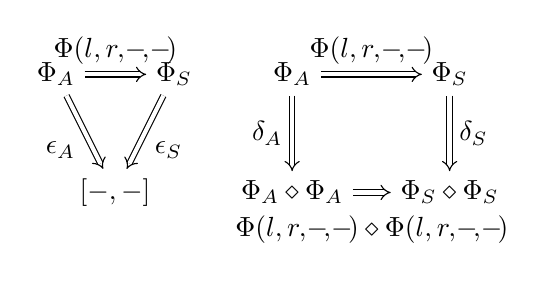
\begin{tikzpicture}[auto]
          \node (pa) at (0, 0) {$\Phi_A$};
          \node (ps) at (1.5, 0) {$\Phi_S$};
          \node (ins) at (0.75, -1.5) {$\inset{-}{-}$};

          \draw[double,double equal sign distance,-implies] (pa) to node{$\Phi(l,r,\!-\!,\!-\!)$}(ps);
          \draw[double,double equal sign distance,-implies] (pa) to node[swap]{$\epsilon_A$}(ins);
          \draw[double,double equal sign distance,-implies] (ps) to node{$\epsilon_S$}(ins);

          \node (pa) at (3, 0) {$\Phi_A$};
          \node (ps) at (5, 0) {$\Phi_S$};
          \node (papa) at (3, -1.5) {$\Phi_A\diamond\Phi_A$};
          \node (psps) at (5, -1.5) {$\Phi_S\diamond\Phi_S$};

          \draw[double,double equal sign distance,-implies] (pa) to node[swap]{$\delta_A$}(papa);
          \draw[double,double equal sign distance,-implies] (ps) to node{$\delta_S$}(psps);
          \draw[double,double equal sign distance,-implies] (pa) to node{$\Phi(l,r,\!-\!,\!-\!)$}(ps);
          \draw[double,double equal sign distance,-implies] (papa) to node[swap,yshift = -5]{$\Phi(l,r,\!-\!,\!-\!)\diamond \Phi(l,r,\!-\!,\!-\!)$}(psps);
         \end{tikzpicture}
      \end{center}
    \end{theorem}
    証明は省略するが、Lawful性の等式とこの二つの図式を米田の補題的に対応させると示せる。
  \end{frame}
  \begin{frame}  
    また射$\Phi(l,r,\!-\!,\!-\!)$の振る舞いはコモナド間の準同型写像のように思えるが、これは実際にプロコモナドの成す圏の特殊な1-cellとなる。\\
    $\alpha = \Phi(l,r,-,-)$として、
    \begin{center}
      \scriptsize
      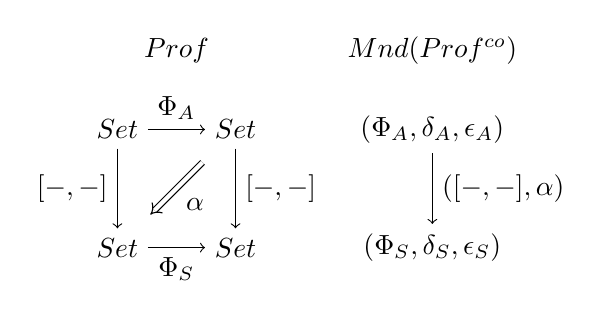
\begin{tikzpicture}[auto]
        \node (c1) at (0.75, 1) {$\cat{Prof}$};

        \node (c1) at (0, 0) {$\cat{Set}$};
        \node (c2) at (1.5, 0) {$\cat{Set}$};
        \node (c3) at (0, -1.5) {$\cat{Set}$};
        \node (c4) at (1.5, -1.5) {$\cat{Set}$};
        \draw[double,double equal sign distance,-implies,shorten >=7pt,shorten <=7pt] (c2) to node{$\alpha$}(c3);
        \draw[->] (c1) to node{$\Phi_A$}(c2);
        \draw[->] (c3) to node[swap]{$\Phi_S$}(c4);
        \draw[->] (c1) to node[swap]{$\inset{-}{-}$}(c3);
        \draw[->] (c2) to node{$\inset{-}{-}$}(c4);
        \node (c1) at (4, 1) {$\cat{Mnd(Prof^{co})}$};
        \node (cma) at (4, 0) {$(\Phi_A,\delta_A,\epsilon_A)$};
        \node (cms) at (4, -1.5) {$(\Phi_S,\delta_S,\epsilon_S)$};
        \draw[->] (cma) to node{$(\inset{-}{-},\alpha)$}(cms);
       \end{tikzpicture}
    \end{center}
    余状態コモナドにおける余代数がwell-behaved lensとなる事実と関係性があるかもしれない。
  \end{frame}
  \begin{frame}
    \frametitle{参考文献}
  
    \bibliographystyle{alpha}
    \bibliography{../bibtex/optics}
  
  \end{frame}

\end{document}

目的自身を抽象化できることは興味ぶかい
興味を優先
2-cateogry を今後の課題に。
まとめを全体の構成と対応。

論点を整理
丹原の別証明